% !TeX program = pdflatex
% !TeX encoding = utf8
% !TeX spellcheck = uk_UA
% !BIB program = bibtex8

\documentclass[18pt]{LectMechanics}
\usetikzlibrary{patterns, snakes}

\tikzset{
	body/.pic = {
		\fill[red!50, draw=red, opacity=0.5]  plot[smooth cycle, tension=.7] coordinates {
			(-1,0)
			(-0.5,1)
			(0.5,2)
			(2.5,1.5)
			(3,0.5)
			(2,-1.5)
			(0.5,-2)
			(-0.5,-1)
		};
	}
}



\usetikzlibrary{arrows.meta}

\title[Physics 1]{\huge\bfseries Dynamics}
\date{}

\begin{document}
%=======================================================================================================
%\usebackgroundtemplate{
%
%\tikz\node[opacity=0.3]{\includegraphics[width=\paperwidth,height=\paperheight]{background}};%
%}
\begin{frame}
	\titlepage
\end{frame}
%=======================================================================================================
\usebackgroundtemplate{
}




%=======================================================================================================
\begin{frame}{Goals for Lecture}{}
	\begin{itemize}
		\item To introduce the concept of force.
		\item To understand the types of interactions in modern physics.
		\item To describe the types of forces in mechanics.
		\item Newtonian laws.
		\item To analize the equation of particle motion and many-particle system.
		\item To understand the Momentum Conservation Law.
	\end{itemize}
\end{frame}
%=======================================================================================================


%=======================================================================================================
\begin{frame}{Newtonian Mechanics}{}\small
	\begin{columns}
		\begin{column}[t]{0.7\linewidth}
			\only<1>{
				The relation between a force and the acceleration it causes was first understood
				by Isaac Newton (1642 –1727). The study of that relation, as Newton presented it, is called \emph{Newtonian mechanics}.
			}
			\only<2>{
				Newtonian mechanics apply if:
				\begin{enumerate}
					\item the velocities of the interacting bodies are very small compared to speed of light $v \ll c = 299 792 458$~m/s;
					\item the interacting bodies are very large then the scale of atomic structure;
					      in an atom)
				\end{enumerate}

				Newtonian mechanics still, it is a very important special case because it applies
				to the motion of objects ranging in size from the very small (almost on the scale of
				atomic structure) to astronomical (galaxies and clusters of galaxies).
			}
		\end{column}
		\begin{column}[t]{0.3\linewidth}
			\begin{center}
				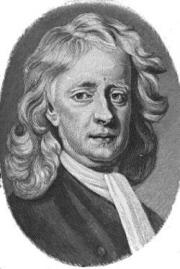
\includegraphics[width=1\linewidth]{Newton}
			\end{center}
		\end{column}
	\end{columns}

\end{frame}
%=======================================================================================================

%=======================================================================================================
\begin{frame}{What is FORCE?}{}
	\only<1>{
		Physical bodyes interact with each other!

		A \emph{force} is an characteristics of interaction between two physical bodyes involving a push or a pull.
	}
	\only<2>{
		The sum of forces acting on a body is called the \emph{total force} or the \emph{net force}. The net force is a single force that replaces the effect of the original forces on the body:
		\begin{equation*}\label{key}
			\vec F_\mathrm{net\, force} = \vec F_1 + \vec F_2 + \vec F_3 +\vec F_4 +\vec F_5
		\end{equation*}
	}
	\begin{center}
		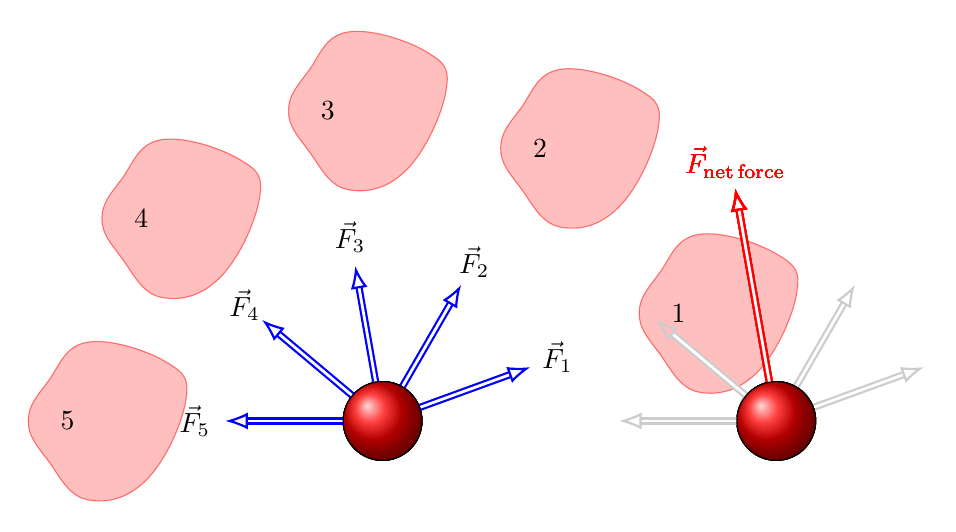
\begin{tikzpicture}
			\foreach \i [count=\n]  in {20,60,...,180} {
			\draw[-{Latex[open]}, thick, blue, double distance=1pt] (0,0) -- (\i:2);
			\node[anchor=\i] at (\i:2.7) {$\vec F_{\n}$};
			\draw[ball color=red] (0,0) circle (0.5);
			\pic<1>[scale=0.5] at (\i:4)  {body};
			\node<1> at (\i:4) {\n};
			%\draw<2>[-{Latex[open]}, thick, red, double distance=1pt] (0,0) +(\i:4) -- (\i:2);
			\draw<2>[-{Latex[open]}, thick, gray!40, double distance=1pt] (5,0) -- +(\i:2);
			\draw<2>[-{Latex[open]}, thick, red, double distance=1pt] (5,0) -- +(100:3) node[above] {$\vec F_\mathrm{net\, force}$};
			\draw<2>[ball color=red] (5,0) circle (0.5) ;
			}
		\end{tikzpicture}
	\end{center}
\end{frame}
%=======================================================================================================

%=======================================================================================================
\begin{frame}{Forces in mechanics}{}\footnotesize
	\only<1>{
		\begin{minipage}{0.7\linewidth}
			\emph{Force of gravity ($m\vec g$)}

			The force of gravity acting on an object due to its mass. An object's weight is directed down, toward the center of the gravitating body; like the Earth or moon, for example.
		\end{minipage}%
		\begin{minipage}{0.3\linewidth}
			\begin{center}
				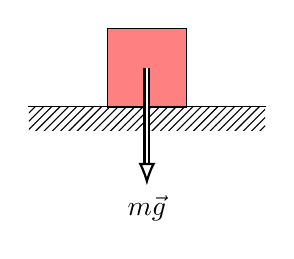
\begin{tikzpicture}
					\tikzstyle{ground}=[fill,pattern=north east lines,draw=none,minimum width=0.75cm,minimum height=0.3cm]
					\node (wall1) [ground, minimum width=3cm,yshift=-0.15cm] {};
					\draw (wall1.north west) -- (wall1.north east);
					\fill[red!50, draw=black] (-0.5,0) rectangle +(1,1);
					\draw[-{Latex[open]}, thick, double distance=1pt] (0,0.5) -- +(0,-1.5) node[below] {$m\vec g$};
				\end{tikzpicture}
			\end{center}%	
		\end{minipage}

		\begin{minipage}{0.7\linewidth}
			\emph{Normal ($\vec N$)}

			The force between two solids in contact that prevents them from occupying the same space. The normal force is directed perpendicular to the surface. A <<normal>> in mathematics is a line perpendicular to a planar curve or surface; thus the name <<normal force>>
		\end{minipage}%
		\begin{minipage}{0.3\linewidth}
			\begin{center}
				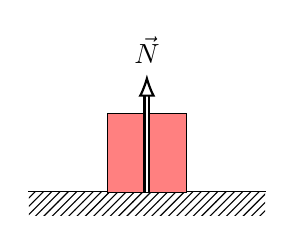
\begin{tikzpicture}
					\tikzstyle{ground}=[fill,pattern=north east lines,draw=none,minimum width=0.75cm,minimum height=0.3cm]
					\node (wall1) [ground, minimum width=3cm,yshift=-0.15cm] {};
					\draw (wall1.north west) -- (wall1.north east);
					\fill[red!50, draw=black] (-0.5,0) rectangle +(1,1);
					\draw[-{Latex[open]}, thick, double distance=1pt] (0,0) -- +(0,1.5) node[above] {$\vec N$};
				\end{tikzpicture}
			\end{center}
		\end{minipage}%

		\begin{minipage}{0.7\linewidth}
			\emph{Friction ($\vec F_f$)}

			The force between solids in contact that resists their sliding across one another. Friction is directed opposite the direction of relative motion or the intended direction of motion of either of the surfaces.
		\end{minipage}%
		\begin{minipage}{0.3\linewidth}
			\begin{center}
				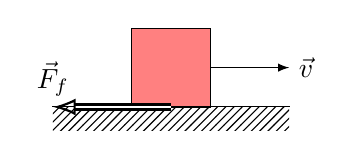
\begin{tikzpicture}
					\tikzstyle{ground}=[fill,pattern=north east lines,draw=none,minimum width=0.75cm,minimum height=0.3cm]
					\node (wall1) [ground, minimum width=3cm,yshift=-0.15cm] {};
					\draw (wall1.north west) -- (wall1.north east);
					\fill[red!50, draw=black] (-0.5,0) rectangle +(1,1);
					\draw[-{Latex[open]}, thick, double distance=1pt] (0,0) -- +(-1.5,0) node[above] {$\vec F_f$};
					\draw[-latex] (0.5,0.5) -- +(1,0) node[right] {$\vec v$};
				\end{tikzpicture}
			\end{center}
		\end{minipage}%
	}
	\only<2>{
		\begin{minipage}{0.7\linewidth}
			\emph{Tension ($\vec T$)}

			The force exerted by an object being pulled upon from opposite ends like a string, rope, cable, chain, etc. Tension is directed along the axis of the object. (Although normally associated with solids, liquids and gases can also be said exert tension in some circumstances.)
		\end{minipage}%
		\begin{minipage}{0.3\linewidth}
			\begin{center}
				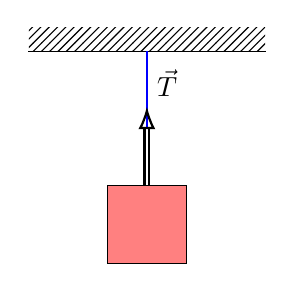
\begin{tikzpicture}
					\tikzstyle{ground}=[fill,pattern=north east lines,draw=none,minimum width=0.75cm,minimum height=0.3cm]
					\node (wall1) [ground, minimum width=3cm,yshift=-0.15cm] {};
					\draw (wall1.south west) -- (wall1.south east);
					\fill[red!50, draw=black] (-0.5,-3) rectangle +(1,1);
					\draw[thick, blue] (0,-0.3) -- (0,-2);
					\draw[-{Latex[open]}, thick, double distance=1pt] (0,-2) -- +(0,1) node[above right] {$\vec T$};
					%		\draw[-latex] (0.5,0.5) -- +(1,0) node[right] {$\vec v$};
				\end{tikzpicture}
			\end{center}
		\end{minipage}%

		\begin{minipage}{0.7\linewidth}
			\emph{Elasticity ($\vec F_e$)}

			The force exerted by an object under deformation (typically tension or compression) that will return to its original shape when released like a spring or rubber band. Elasticity, like tension, is directed along an axis (although there are exceptions to this rule).
		\end{minipage}%
		\begin{minipage}{0.3\linewidth}
			\begin{center}
				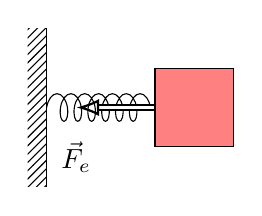
\begin{tikzpicture}
					\tikzstyle{ground}=[fill,pattern=north east lines,draw=none,minimum width=0.3,minimum height=0.6]

					\node (wall1) [ground, minimum height=2cm] {};
					\draw (wall1.north east) -- (wall1.south east);
					\node [draw,minimum width=1cm,minimum height=1cm, fill=red!50] (mass) at (2,0) {};
					\node (fix) at (0,0) {};
					\draw [
						snake=coil,
						segment amplitude=5pt,
						segment length=5pt
					] (wall1.east) -- (mass);
					\draw[-{Latex[open]}, thick, double distance=1pt] (mass) -- +(-1.5,0) node[below=0.3cm] {$\vec F_e$};
				\end{tikzpicture}
			\end{center}
		\end{minipage}%
	}
\end{frame}
%=======================================================================================================

%=======================================================================================================
\begin{frame}{Fundamental forces}{}\footnotesize
	All the forces in the universe can be explained in terms of the following four fundamental interactions.
	\begin{enumerate}
		\item Gravity

		      The interaction between objects due to their mass. Weight is a synonym for the force of gravity.
		\item Electromagnetism

		      The interaction between objects due to their charge. All the forces discussed above are electromagnetic in origin except weight.

		\item Strong Nuclear Interaction

		      The interaction between subatomic particles with "color" (an abstract quantity that has nothing to do with human vision). This is the force that holds protons and neutrons together in the nucleus and holds quarks together in the protons and neutrons. It cannot be felt outside of the nucleus.

		\item Weak Nuclear Interaction

		      The interaction between subatomic particles with "flavor" (an abstract quantity that has nothing to do with human taste). This force, which is many times weaker than the strong nuclear interaction, is involved in certain forms of radioactive decay.
	\end{enumerate}
\end{frame}
%=======================================================================================================

%=======================================================================================================
\begin{frame}{What is MASS?}{}

	Experience shows that every body <<resists>> any effort to change its velocity, both in magnitude and
	direction. This property expressing the degree of unsusceptibility of a body to any change in its velocity is called inertness. Different bodies reveal this property in different degrees.

	A measure of inertness is provided by the quantity called \emph{mass}. A body possessing a greater mass is more inert, and vice versa.

	The basic SI unit of mass is the kilogram (kg).

	\begin{minipage}{0.5\linewidth}
		The notion of mass $m$ by defining the ratio of masses of two different bodies via the inverse ratio of accelerations imparted to them by equal forces:
		\begin{equation*}
			\frac{m_1}{m_2} = \frac{a_2}{a_1}.
		\end{equation*}
	\end{minipage}%
	\begin{minipage}{0.5\linewidth}
		\begin{center}
			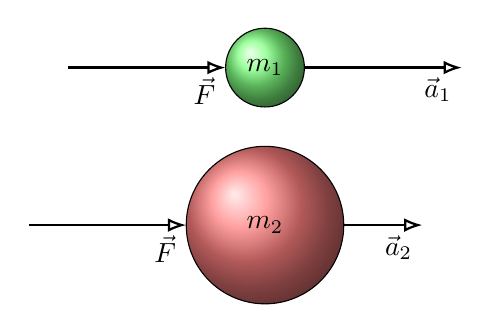
\begin{tikzpicture}
				\draw[-{Latex[open]}, thick] (0,0) -- +(2,0) node[below left] {$\vec F$};
				\draw[ball color=green!50] (2.5,0) circle (0.5) node[] {$m_1$};
				\draw[-{Latex[open]}, thick] (3,0) -- +(2,0) node[below left] {$\vec a_1$};
				\begin{scope}[yshift=-2cm]
					\draw[-{Latex[open]}, thick] (-0.5,0) -- +(2,0) node[below left] {$\vec F$};
					\draw[ball color=red!50] (2.5,0) circle (1) node[] {$m_2$};
					\draw[-{Latex[open]}, thick] (3.5,0) -- +(1,0) node[below left] {$\vec a_2$};
				\end{scope}
			\end{tikzpicture}
		\end{center}
	\end{minipage}


\end{frame}
%=======================================================================================================

%=======================================================================================================
\begin{frame}{Properties of MASS}{}
	\begin{enumerate}
		\item mass is an \emph{additive quantity}, i.e. the mass of a
		      composite body is equal to the sum of the masses of its constituents;
		      \begin{equation*}
			      m_1 + m_2 + m_3 + m_4 = m
		      \end{equation*}
		      \begin{center}
			      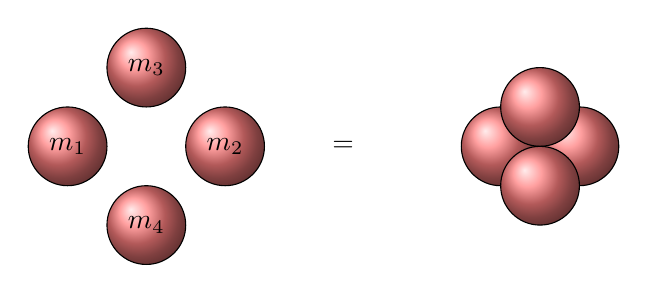
\begin{tikzpicture}
				      \draw[ball color=red!50] (-1,0) circle (0.5) node {$m_1$};
				      \draw[ball color=red!50] (1,0) circle (0.5) node {$m_2$};
				      \draw[ball color=red!50] (0,1) circle (0.5) node {$m_3$};
				      \draw[ball color=red!50] (0,-1) circle (0.5) node {$m_4$};

				      \node at (2.5,0) {$=$};
				      \begin{scope}[xshift=5cm]
					      \draw[ball color=red!50] (-0.5,0) circle (0.5);
					      \draw[ball color=red!50] (0.5,0) circle (0.5);
					      \draw[ball color=red!50] (0,0.5) circle (0.5);
					      \draw[ball color=red!50] (0,-0.5) circle (0.5);
				      \end{scope}
			      \end{tikzpicture}
		      \end{center}
		\item the mass of a body proper is a constant quantity, remaining invariable in the process of motion.
	\end{enumerate}
\end{frame}
%=======================================================================================================

%=======================================================================================================
\begin{frame}{Linear Momentum}{}
	In Newtonian mechanics, linear momentum, translational momentum, or simply momentum is the product of the mass and velocity of an object. It is a three-dimensional vector quantity, possessing a magnitude and a direction. If m is an object's mass and v is the velocity (also a vector), then the momentum is

	\begin{equation*}
		\vec p = m\vec v
	\end{equation*}

	In SI units, it is measured in kilogram meters per second (kg$\cdot$m/s).
\end{frame}
%=======================================================================================================

%=======================================================================================================
\begin{frame}{Inertial frame of reference}{Newton First Law}
	There is a reference frame
	in which acceleration of a mass point arises solely due to its
	interaction with other bodies. Then a \textbf{free mass point
		experiencing no action from any other bodies moves rectilinearly and uniformly, relative to such a frame}, or, in other
	words, due to inertia. Such a \emph{reference frame is called inertial}.

	The statement of the existence of inertial reference
	frames formulates the content of the \textbf{first law of classical
		mechanics}, the law of inertia of Galileo and Newton.
\end{frame}
%=======================================================================================================


%=======================================================================================================
\begin{frame}{Newton Second Law}{}
	Product of the mass of a particle by its acceleration is equal to the net force acting on it:
	\begin{equation*}
		\tcbhighmath[drop fuzzy shadow]{m\vec a = \vec F}
	\end{equation*}
	This equation is referred to as the motion equation of a particle.

\end{frame}
%=======================================================================================================

%=======================================================================================================
\begin{frame}[t]{Newton Third Law}{}
	\begin{columns}
		\begin{column}{0.4\linewidth}
			Two mass points act on each other with forces which are always
			equal in magnitude and oppositely directed along a straight
			line connecting these points:
			\begin{equation*}
				\tcbhighmath[drop fuzzy shadow]{\vec F_{12} = - \vec F_{21}}
			\end{equation*}
			This implies that interaction forces always appear in pairs.
			The two forces are applied to different mass points; besides,
			they are the forces of the same nature.
		\end{column}
		\begin{column}{0.6\linewidth}
			\begin{center}
				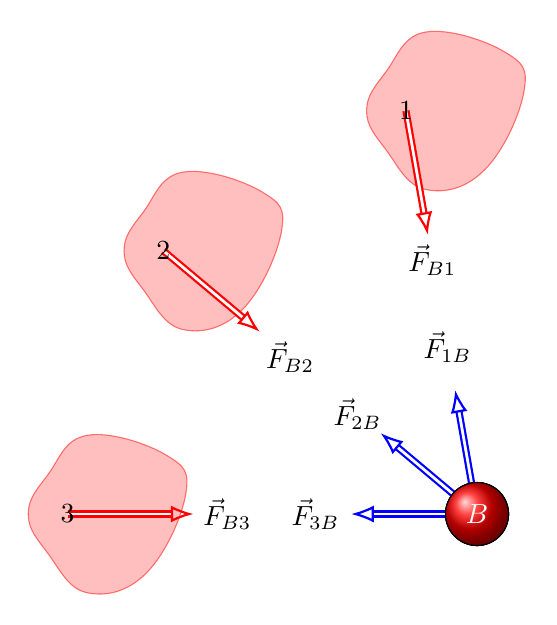
\begin{tikzpicture}[scale=0.8]
					\pgfmathsetmacro{\dist}{6.5}
					\foreach \i [count=\n]  in {100,140,...,180} {
					\draw[-{Latex[open]}, thick, blue, double distance=1pt] (0,0) -- (\i:2);
					\node[anchor=\i] at (\i:3.1) {$\vec F_{\n B}$};
					\draw[ball color=red] (0,0) circle (0.5) node[color=white] {$B$};
					\pic[scale=0.5] at (\i:\dist)  {body};
					\draw[-{Latex[open]}, thick, red, double distance=1pt] (0,0) +(\i:\dist) -- (\i:\dist-2);
					\node[anchor=\i] at (\i:\dist-2) {$\vec F_{B\n}$};
					\node at (\i:\dist) {\n};
					}
				\end{tikzpicture}
			\end{center}
		\end{column}
	\end{columns}

\end{frame}
%=======================================================================================================

%=======================================================================================================
\begin{frame}[t]{Examples}{Body diagram of an an object in inclined plane}
	\begin{columns}
		\begin{column}{0.4\linewidth}\footnotesize
			Newton Second Low for the body $m_1$:
			\begin{equation*}
				m_1\vec a = m_1\vec g + \vec N + \vec F_f
			\end{equation*}
			Projections
			\begin{align*}
				OX: \, & m_1 a = m_1 g\sin\alpha - F_f \\
				OY: \, & 0 = N - m_1 g\cos\alpha
			\end{align*}

			Newton Second Low for the body $m_2$:
			\begin{equation*}
				m_2\vec a = m_2\vec g + \vec T
			\end{equation*}
			Projections
			\begin{equation*}
				OY: m_2 a  = T - m_2 g
			\end{equation*}
		\end{column}
		\begin{column}{0.6\linewidth}
			\begin{center}
				\begin{tikzpicture}
					\pgfmathsetmacro{\h}{3}
					\pgfmathsetmacro{\l}{4}
					\pgfmathsetmacro{\incangle}{atan(\h/\l)}
					\pgfmathsetmacro{\R}{0.5}
					\coordinate (R) at (\incangle:5.5);
					\fill[red!50, draw=black] (0,0) -- ++(\l,0) -- ++(0,\h) coordinate(A) -- cycle;
					\draw[-latex] (0,0) +(0:0.5) arc (0:\incangle:0.5) node[pos=0.5, right] {$\alpha$};
					\coordinate (RT1) at  ([shift={(135:\R)}]R);
					\coordinate (RT2) at  ([shift={(0:\R)}]R);
					\draw[fill=gray, thick] (R) circle (\R)
					circle (\R-0.1)
					circle (0.05);
					\path (0,0) -- (A) coordinate[pos=0.3] (B);
					\draw[fill=blue!50, rotate=\incangle] (B) rectangle  +(1,1) [add reference=BP1];
					\draw (BP1 east) -- (RT1);
					\draw[fill=blue!50] ([shift={(-0.5,-3)}]RT2) rectangle  +(1,1) [add reference=BP2];
					\draw (BP2 north) -- (RT2);
					% ========== Forces ======================
					\draw[-latex, thick] (BP1 center) -- +(-90:2) coordinate (G1) node[below] {$m_1\vec g$};
					\draw[dashed] (BP1 center) -- +(\incangle-90:{2*cos(\incangle)}) coordinate (G2);
					\draw (BP1 center)  +(-90:0.75) arc(-90:\incangle-90:0.75) node[pos=0.5, below] {$\alpha$}; 
					\draw[-latex, thick, green!50!black] (BP1 south) -- ([shift={({90+\incangle}:2)}]BP1 south) node[above] {$\vec N$};
					\draw[-latex, thick] (BP1 south) -- ([shift={(\incangle:1)}]BP1 south) node[below right] {$\vec F_f$};

					\draw[-latex, thick, green!50!black] (BP2 north) -- ([yshift=1cm]BP2 north) node[right] {$\vec T$};
					\draw[-latex, thick] (BP2 center) -- ([yshift=-1.5cm]BP2 center) node[right] {$m_2\vec g$};
					\draw[dashed] (G1) -- (G2);
					% ========== Axes ======================
					\begin{scope}[rotate=\incangle, shift={(5,1)}]
						\draw[dashed, gray, -latex] (0,0) -- +(-2,0) node[left] {$+x$};
						\draw[dashed, gray, -latex] (0,0) -- +(0,1.5) node[above] {$+y$};
					\end{scope}
					\draw[dashed, gray, -latex, shift={(6,1)}] (0,0) -- +(0,2) node[above] {$+y$};

					% ====== Labels for Bodyes
					\node[white] at (BP1 center) {$1$};
					\node[white] at (BP2 center) {$2$};
				\end{tikzpicture}
			\end{center}
		\end{column}
	\end{columns}
\end{frame}
%=======================================================================================================

%=======================================================================================================
\begin{frame}{The system of particles}{}
	\framesubtitle<5>{The Law of Particle System Motion}
	\framesubtitle<6-7>{The Law of Linear Momentum Conservation}
	\begin{columns}
		\begin{column}{0.4\linewidth}\small
			\only<1-2>{
			Consider now a system of $N$ particles of masses $m_1, m_2, \ldots, m_N$.
			The total mass is
			\begin{equation*}
				M = m_1 + m_2 + \ldots + m_N
			\end{equation*}
			
				Each particle can be represented by its location $\vec r_{i}$,
			}
			\only<2>{
				velocity $\vec v_{i}$ and linear momentum $m_i \vec v_{i}$.

				The system as a whole has a total linear momentum $\vec P$, which is defined to be the vector sum of the individual particle linear momenta:
				\begin{equation*}
					\vec P = m_1 \vec v_{1} + m_2 \vec v_{2} + \ldots + m_N \vec v_{N}
				\end{equation*}
			}
			\only<3>{
			Let’s extend our system to two interacting objects, for example the cart and the spring.
			The forces between the spring and cart are now internal forces. Both objects, the cart and
			the spring, experience these internal forces, which by Newton’s Third Law are equal in
			magnitude and applied in opposite directions. So when we sum up the internal forces for
			the whole system, they cancel. Thus the sum of all the internal forces is always zero,
				\begin{equation*}
				\sum \vec F_{ij} = 0
				\end{equation*}
			}
		\only<4>{
			External forces are acting on our system $\vec F^{ext}$; the gravitational force, the contact force
			between the inclined plane and the cart, and also a new external force, the force between
			the spring and the force sensor. The force acting on the system is the sum of the internal
			and the external forces. However, as we have shown, the internal forces cancel, so we
			have the total force acting on system equal to:
			\begin{equation*}
			\vec F = \sum \vec F^{ext} 
			\end{equation*}
			}
		\only<5>{
		The time \emph{derivative of the momentum of a system} is equal to the vector sum of all \emph{external forces} 
		acting on the particles of the system:
		\begin{equation*}
			\tcbhighmath[drop fuzzy shadow]{\frac{d\vec P}{dt} = \vec F^{ext}.}
		\end{equation*} 
		In accordance with this equation the momentum of a system may vary only due to \emph{external forces}.
		Internal forces cannot change the momentum, of a system.  
		}
		\only<6>{
		 Closed system is a physical system that doesn't exchange any matter with its surroundings, and isn't subject to any net force whose source is external to the system:
		 \begin{equation*}\label{key}
			 \tcbhighmath[drop fuzzy shadow]{\vec F^{ext} = 0.}
		 \end{equation*}
		}
		\only<7>{
			 From the Law of Particle System Motion
			 \begin{equation*}
			 \tcbhighmath[drop fuzzy shadow]{\frac{d\vec P}{dt} = 0.}
			 \end{equation*}  
			follows  the law of momentum conservation: 
			in an inertial reference frame the momentum of a closed system of particles 
			remains constant, i.e. does not change in the course of time: 
			\begin{equation*}
			\tcbhighmath[drop fuzzy shadow]{\vec P = \mathrm{const}.}
			\end{equation*} 
			} 
		\end{column}
		\begin{column}{0.6\linewidth}
			\begin{overprint}
				\begin{tikzpicture}[scale=0.8, every node/.style={scale=0.8}]
					\draw[-latex, gray, thick] (0,0) -- +(1,0) node[right] {$y$};
					\draw[-latex, gray, thick] (0,0) -- +(0,1) node[right] {$z$};
					\draw[-latex, gray, thick] (0,0) -- +(-135:1) node[right] {$x$};
					\coordinate (B1) at (1,3);
					\coordinate (B2) at (4,5);
					\coordinate (B3) at (7,3);
					\coordinate (B4) at (4,1);

					\foreach \i in {1,...,4} {
							\draw[ball color=red!50] (B\i) circle (0.1);
							\draw<1-2>[-latex, gray] (0,0) -- node[below] {$\vec r_{\i}$} (B\i);
							\draw<2->[-latex, green!50!black] (B\i) -- +({180-30*\i}:1) node[above right] {$m_{\i}\vec v_{\i}$};

							\foreach \j in {1,...,4} {
									\ifnum\i=\j
										\relax
									\else
										\draw<3->[-latex, blue] (B\i) -- ($(B\i)!1cm!(B\j)$) node[pos=1.3] {$\vec F_{\i\j}$};
										\draw<3->[-latex, blue] (B\j) -- ($(B\j)!1cm!(B\i)$);
									\fi
								}
							\draw<4-5>[-latex, red, thick] (B\i) -- +(260:1.7) node[pos=1.1] {$\vec F^{ex}$};
						}

				\end{tikzpicture}
			\end{overprint}
		\end{column}
	\end{columns}
\end{frame}
%=======================================================================================================

%=======================================================================================================
\begin{frame}{The low of Linear Momentum Conservation}{}\small
Sometimes in a non-closed system it is not the momentum $\vec P$ itself that remains constant, but its $P_x$ projection on a certain $x$ direction. This happens when 
the projection of the resultant $\vec F^{ext}$ of the external forces on 
the $x$ direction is equal to zero, i.e. the vector $\vec F^{ext}$ is  
perpendicular to that direction, for example, if $F_x^{ext} = 0$
whence it follows that if \emph{$P_x = \mathrm{const}$}. 

For example, when a system moves in a uniform field of gravity, 
the projection of its momentum on any horizontal direction 
remains constant whatever happens inside the system. 
\begin{center}
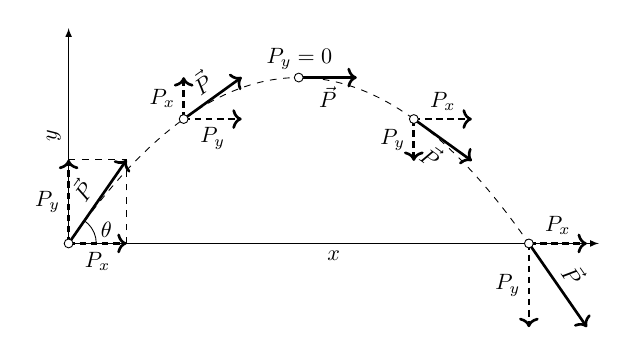
\begin{tikzpicture}[scale=0.8, transform shape]  %projectile motion
\begin{axis}[
width=10cm, %set bigger width
height=5cm,
xmin=0,xmax=11.5,
ymin=0,ymax=4,
xlabel=$x$,
ylabel=$y$,
axis x line = bottom,
axis y line = left,
axis line style={-latex},
%axis on top,
ticks = none,clip=false,
]

\tikzset{every mark/.append style={fill=white}}

%variable definitions
\def\g{-9.8} %gravity
\def\v{10} %velocity
\def\ang{51} %angle
\def\s{0.2}
\pgfmathsetmacro{\t}{0}
%flight path
\addplot[
dashed,
domain=0:10,
samples=100,]
{{\g*(x^2)/(2*\v^2*cos(\ang)^2)+x*tan(\ang)}}
node[midway,above]{$P_y=0$};

%vector at start
\coordinate (A) at (axis cs: {\v*cos(\ang)*\t}, {\v*\t*sin(\ang)+0.5*\g*(\t^2)});
\coordinate (B) at (axis cs: {\v*cos(\ang)*\t+\s*\v*cos(\ang)}, {\v*\t*sin(\ang)+0.5*\g*\t^2+\s*(\v*sin(\ang)+\g*\t)});
\draw[very thick,->](A)--(B)
node[midway,sloped,above]{$\vec P$};
\draw[densely dashed,very thick,->](A)--(B|-A)
node[midway,below]{$P_x$};
\draw[densely dashed,very thick,->](A)--(B-|A)
node[midway,left]{$P_y$};

\path plot[mark=*] coordinates {(A)};

%dashed box around start vector
\draw[dashed](B-|A)--(B);
\draw[dashed](B|-A)--(B);

%vector at end
\pgfmathsetmacro{\a}{{-1*(2/\g)*\v*sin(\ang)}}
\coordinate (E) at (axis cs:{\v*cos(\ang)*\a},{\v*\a*sin(\ang)+0.5*\g*(\a^2)}){};
\coordinate (F) at (axis cs:{\v*cos(\ang)*\a+\s*\v*cos(\ang))}, {\v*\a*sin(\ang)+0.5*\g*\a^2+\s*(\v*sin(\ang)+\g*\a)});
\draw[very thick,->](E)--(F)
node[midway,sloped,above]{$\vec P$};
\draw[densely dashed,very thick,->](E)--(F |- E)
node[midway,above]{$P_x$};
\draw[densely dashed,very thick,->](E)--(F-| E)
node[midway,left]{$P_y$};

\path plot[mark=*] coordinates {(E)};

%vector 1/2 up
\pgfmathsetmacro{\b}{{(-1*(2/\g)*\v*sin(\ang))/4}}
\coordinate (H) at (axis cs:{\v*cos(\ang)*\b},{\v*\b*sin(\ang)+0.5*\g*(\b^2)});
\coordinate (I) at (axis cs: {\v*cos(\ang)*\b+\s*\v*cos(\ang)},{\v*\b*sin(\ang)+0.5*\g*\b^2+\s*(\v*sin(\ang)+\g*\b)});
\draw[very thick,->](H)--(I)
node[midway,sloped,above]{$\vec P$};
\draw[densely dashed,very thick,->](H)--(I-|H)
node[midway,left]{$P_x$};
\draw[densely dashed,very thick,->](H)--(I|-H)
node[midway,below]{$P_y$};

\path plot[mark=*] coordinates {(H)};

%vector halfway
\pgfmathsetmacro{\c}{{(-1*(2/\g)*\v*sin(\ang))/2}}
\coordinate (L) at (axis cs:{\v*cos(\ang)*\c},{\v*\c*sin(\ang)+0.5*\g*(\c^2)});
\coordinate (M) at (axis cs:{\v*cos(\ang)*\c+\s*\v*cos(\ang))},{\v*\c*sin(\ang)+0.5*\g*\c^2+\s*(\v*sin(\ang)+\g*\c)});
\draw[very thick,->](L)--(M)
node[midway,sloped,below]{$\vec P$};


%T2 line; halfway up flight path
%\draw[loosely dashed] (L) -- (axis cs:{\v*cos(\ang)*\c},0)
%node[midway,right] {$\frac{t_\text{total}}{2}$};


\path plot[mark=*] coordinates {(L)};

%vector 1/2 down
\pgfmathsetmacro{\d}{{(-1*(2/\g)*\v*sin(\ang))*0.75}}
\coordinate (P) at (axis cs:{\v*cos(\ang)*\d},{\v*\d*sin(\ang)+0.5*\g*(\d^2)});
\coordinate (Q) at (axis cs:{(\v*cos(\ang)*\d+\s*\v*cos(\ang))},{\v*\d*sin(\ang)+0.5*\g*\d^2+\s*(\v*sin(\ang)+\g*\d)});
\draw[very thick,->](P)--(Q)
node[midway,sloped,below]{$\vec P$};
\draw[densely dashed,very thick,->](P)--(Q|-P)
node[midway,above]{$P_x$};
\draw[densely dashed,very thick,->](P)--(Q-|P)
node[midway,left]{$P_y$};

\path plot[mark=*] coordinates {(P)};

%start vector angle label
\node[circle,minimum size=25pt] at (A) (circ) {};
\node[right] at (circ.30) {$\theta$};
\path[clip] (A) -- (B) -- (B|-A) -- cycle;
\node[circle,draw,minimum size=25pt] at (A) (circ) {};
\end{axis}
\end{tikzpicture}
\end{center}

\end{frame}
%=======================================================================================================

\end{document}